%% 
%% This is a sample doctoral dissertation.  It shows the appropriate
%% structure for your dissertation.  It should handle most of the
%% strange requirements imposed by the Grad school; like the different
%% handling of titles of one/many appendices.  It will automatically
%% handle the linespacing changes.  The body default is double-spaced
%% (except when you use the singlespace or condensed options).  The
%% default for quotations is single-space, and the default for tabular
%% environments is also single-space.  
%%
%% This class adds the following commands and environments to the
%% report class, upon which it is based:
%% Commands
%% ------------
%% \degree{name}{abbrv} -- Sets the name and abbreviation for the degree.
%%                         These default to ``Doctor of Philosopy''
%%                         and ``Ph.D.'', respectively.
%% \copyrightyear{year} -- for the copyright page.
%% \bachelors{degree}{institution} -- for the abstract
%% \masters{degree}{institution}   --  "
%%     if you have other degrees you may use
%% \secondbachelors{degree}{institution}
%% \thirdbachelors{degree}{institution}
%% \secondmasters{degree}{institution}
%% \thirdmasters{degree}{institution}
%% \priordoctorate{degree}{institution}
%%
%% \committeechair{name}           -- for the signature page
%% or, if you have two co-chairs:
%% \cochairs{first name}{second name}
%%
%% \firstreader{name}              --  "
%% \secondreader{name}             --  "
%% \thirdreader{name}              -- (optional)
%% \fourthreader{name}             --  "
%% \fifthreader{name}              --  "
%% \sixthreader{name}              --  "
%% \departmentchair{name}          -- for the signature page
%% \departmentname{name}           --  "
%%
%% \copyrightpage                  -- produces the copyright page
%% \signaturepage                  -- produces the signature page
%%
%% \frontmatter                    -- these are required in their various
%% \mainmatter                     -- appropriate locations
%% \backmatter                     --
%%
%% \unnumberedchapter[toc]{name}   -- like \chapter, except that it
%%                                    produces an unnumbered chapter;
%%                                    alternatively, like \chapter*,
%%                                    except that it lists the chapter
%%                                    in the table of contents.
%%
%% New environments:
%%   dedication  -- for the dedication
%%   abstract    -- for the abstract
%%
%% The thesis documentclass is built on top of the report document class.
%% It accepts all of the options that the report class accepts, plus the
%% following:
%%     doublespace -- the default, indicates double spacing as per U.Mass.
%%                    requirements.  You will need this when you do your
%%                    final copy.
%%     singlespace -- for earlier work, not acceptable to the Grad school
%%     condensed   -- for earlier work, not acceptable to the Grad school,
%%                    creates condensed versions of the frontmatter. 
%%                    Condensed implies singlespace.
%%     dissertation - the default, indicates that this document is a
%%                    dissertation.
%%     proposal    -- indicates that this document is a dissertation proposal,
%%                    rather than a dissertation.  This will only change the
%%                    wording on the title and signature pages.
%%     thesis      -- indicates that this document is a Master's thesis 
%%                    rather than a doctoral dissertation.  This also changes
%%                    the default for \degree to Master of Science, M.S.
%%     allowlisthypenation -- (the default), allows hyphenation of words in
%%                    the table of contents, the list of figures, and the list
%%                    of tables.  I believe that this is acceptable to the 
%%                    Graduate School.
%%     nolisthyphenation -- disallows hyphenation of words in the table of
%%                    contents and the list of figures and tables.  Use this 
%%                    option if the Grad School doesn't like your hyphenation.
%%     nicerdraft  -- relaxes some of the Grad School's rules for working with
%%                    drafts -- has no effect when doublespace is in effect
%%     nonicerdraft -- the default, leaves things in draft as they will be in
%%                     the final version
%% umthesis changes the default font size to 12pt, but you may specify 10pt or
%%   11pt in the options.
\documentclass[proposal]{umthesis}          % for Ph.D. dissertation or proposal
%\documentclass{umthesis}          % for Ph.D. dissertation or proposal
% \documentclass[thesis]{umthesis}  % for Master's thesis

\usepackage{subfigure}
\usepackage{listings}
\usepackage{graphicx}
\usepackage{url}

%\lstset{ %
% language=C,                    % choose the language of the code
% basicstyle=\footnotesize,       % the size of the fonts that are used for the code
%numbers=left,                   % where to put the line-numbers
%numberstyle=\footnotesize,      % the size of the fonts that are used for the line-numbers
%stepnumber=1,                   % the step between two line-numbers. If it is 1 each line will be numbered
%numbersep=5pt,                  % how far the line-numbers are from the code
%backgroundcolor=\color{white},  % choose the background color. You must add \usepackage{color}
%showspaces=false,               % show spaces adding particular underscores
%showstringspaces=false,         % underline spaces within strings
%showtabs=false,                 % show tabs within strings adding particular underscores
%frame=single,           % adds a frame around the code
%tabsize=2,          % sets default tabsize to 2 spaces
%captionpos=b,           % sets the caption-position to bottom
%breaklines=true,        % sets automatic line breaking
%breakatwhitespace=false    % sets if automatic breaks should only happen at whitespace
%escapeinside={\%*}{*)}          % if you want to add a comment within your code
%}

%%
%% If you have enough figures or tables that you run out of space for their
%% numbers in the List of Tables or List of figures, you can use the following
%% command to adjust the space left for numbers.  The default is shown:
%%
%% \setlength{\tablenumberwidth}{2.3em}
\newcommand{\dthreads}{{\scshape Dthreads}}
\newcommand{\Dthreads}{{\scshape Dthreads}}
\newcommand{\Grace}{{\scshape Grace}}
\newcommand{\grace}{{\scshape Grace}}
\newcommand{\Sheriff}{{\scshape Sheriff}}
\newcommand{\sheriff}{{\scshape Sheriff}}
\newcommand{\SheriffProtect}{\textsc{Sheriff-Protect}}
\newcommand{\sheriffProtect}{\textsc{Sheriff-Protect}}
\newcommand{\sheriffprotect}{\textsc{Sheriff-Protect}}
\newcommand{\SheriffDetect}{\textsc{Sheriff-Detect}}
\newcommand{\sheriffDetect}{\textsc{Sheriff-Detect}}
\newcommand{\sheriffdetect}{\textsc{Sheriff-Detect}}
\newcommand{\stopgap}{\textsc{StopGap}}
\newcommand{\Stopgap}{\textsc{StopGap}}
\newcommand{\StopGap}{\textsc{StopGap}}
\newcommand{\pthreads}{\texttt{pthreads}}
\newcommand{\redline}{\textsc{redline}}
\newcommand{\Redline}{\textsc{redline}}


\begin{document}

%%
%% You must fill in all of these appropriately
\title{Safe and Efficient Multithreading}
\author{Tongping Liu}
\date{January 2013} % The date you'll actually graduate -- must be
                     % February, May, or September
\copyrightyear{2013}
\bachelors{B.S.}{Harbin Institute of Technology}
\masters{M.E.}{Huazhong University of Science and Technology}
\secondmasters{M.S.}{UNIVERSITY OF MASSACHUSETTS AMHERST}
%\priordoctorate{Ph.D.}{UNIVERSITY OF MASSACHUSETTS AMHERST}
\committeechair{Emery D. Berger}
\firstreader{Scott F. H. Kaplan}
\secondreader{Yuriy Brun}
%{Yannis Smaragdakis}
\thirdreader{Israel Koren}   % Optional
%\fifthreader{}            % Optional
%\sixthreader{}            % Optional
\departmentchair{Lori A. Clarke}
\departmentname{Department of Computer Science}

%% If your degree is something other than a Ph.D. (for a dissertation), or
%% an M.S. (for a thesis), you will need to uncomment the appropriate
%% following line:
%%
%% \degree{Doctor of Education}{Ed.D.}
%% \degree{Doctor of Philosophy}{Ph.D.}
%%
%% \degree{Master of Arts}{M.A.}
%% \degree{Master of Arts in Teaching}{M.A.T.}
%% \degree{Master of Business Administration}{M.B.A.}
%% \degree{Master of Education}{M.Ed.}
%% \degree{Master of Fine Arts}{M.F.A.}
%% \degree{Master of Landscape Architecture}{M.L.A.}
%% \degree{Master of Music}{M.M.}
%% \degree{Master of Public Administration}{M.P.A.}
%%\degree{Master of Public Health}{M.P.H.}
%% \degree{Master of Regional Planning}{M.R.P.}
%% \degree{Master of Science}{M.S.}
%% \degree{Master of Science in Accounting}{M.S. Acctg.}
%% \degree{Master of Science in Chemical Engineering}{M.S. Ch.E.}
%% \degree{Master of Science in Civil Engineering}{M.S.C.E.}
%% \degree{Master of Science in Electrical and Computer Engineering}{M.S.E.C.E.}
%% \degree{Master of Science in Engineering Management}{M.S. Eng. Mgt.}
%% \degree{Master of Science in Environmental Engineering}{M.S. Env. E.}
%% \degree{Master of Science in Industrial Engineering and Operations Research}{M.S.I.E.O.R.}
%% \degree{Master of Science in Manufacturing Engineering}{M.S. Mfg. Eng.}
%% \degree{Master of Science in Mechanical Engineering}{M.S.M.E.}
%%
%% \degree{Professional Master of Business Administration}{P.M.B.A.}


%%
%% These lines produce the title, copyright, and signature pages.
%% They are Mandatory; except that you could leave out the copyright page
%% if you were preparing an M.S. thesis instead of a PhD dissertation.
\frontmatter
\maketitle
\copyrightpage     %% not required for an M.S. thesis
\signaturepage

%%
%% Dedication is optional -- but this is how you create it
%\begin{dedication}              % Dedication page
%  \begin{center}
%   \emph{ XXXXXX }       
%  \end{center}
%\end{dedication}

%%
%% Epigraph goes here...(aka frontispiece)
%% \chapter{Epigraph}?????

%%
%% Acknowledgements are optional...yeah, right.
%  \chapter{Acknowledgments}             % Acknowledgements page
%  Thanks to all those fine shepherds. Not to mention all the great
%  border collies and suchlike fine animals.

%%
%% Abstract is MANDATORY. -- Except for MS theses

\begin{abstract}                % Abstract
The advent of multicore architecture has increased the demand for multithreaded
programs, but writing them remains painful for programmers. 
It is notoriously far more challenging to write concurrent programs correctly and 
efficiently than sequential ones because of the wide range of performance problems and 
concurrency errors, including false sharing, race conditions, deadlocks, etc. 

In this proposal we introduce a series of runtime systems to combat performance problems and 
concurrency errors of multithreaded problems.
The first system, \Sheriff{}, attacks the notorious performance problem of 
multithreaded programs, false sharing. \Sheriff{} can precisely detect false 
sharing problems without false positives and automatically mitigate false sharing 
problems without user intervention. 
The second system, \dthreads{}, automatically ensures determinism for unmodified C/C++
applications without requiring programmer intervention. \dthreads{} leverages virtual 
memory and process isolation, combined with a deterministic commit protocol, 
to ensure robust deterministic execution with very low runtime overhead.
Finally, we propose \stopgap{}, a novel detection tool for write-write races based on synchronization
 boundaries.
\stopgap{} detects more races than the standard happens-before
approaches without introducing false positives, unlike lockset based approaches.
\stopgap{} can also locate those heap-based overflows and 
underflows without adding perceptible performance overhead.

\end{abstract}

%%
%% Preface goes here...would be just like Acknowledgements -- optional
%% \chapter{Preface} 
%% ...


%%
%% Table of contents is mandatory, lists of tables and figures are 
%% mandatory if you have any tables or figures; must be in this order.
\tableofcontents                % Table of contents
%\listoftables                   % List of Tables
\listoffigures                  % List of Figures

%%
%% We don't handle List of Abbreviations
%% We don't handle Glossary

%%%%%%%%%%%%%%%%%%%%%%%%%%%%%%%%%%%%%%%%%%%%%%%%%%%%%%%%%%%%%%%%%%%%%%%%%
%% Time for the body of the dissertation
\mainmatter   %% <-- This line is mandatory

%%
%% If you want an introduction, which is not a numbered chapter, insert
%% the following two lines.  This is OPTIONAL:
\unnumberedchapter{Introduction}
%False sharing problem is a cache usage problem. 
%Cache, with much faster access speed than main memory, is normally utilized by CPU
%to accelerate program executions by preloading a fixed size of data into the cache each time, 
%called as a cache line.  

%%%%%%%%%%%%%%%%%%%%%%%%%%%%%%%%%%%%%%%%
% Why 
%%%%%%%%%%%%%%%%%%%%%%%%%%%%%%%%%%%%%%%%
\label{sec:intro} 
False sharing is notorious for performance degradation in multithreaded
programs due to cache coherence protocol, which exists in most mordern 
 mutlicore processors.
The reason of having cache coherence protocol is to ensure the correctness of
program executions: 
if some cache line data on a core needs to be updated, the duplicated data in any other core's private 
cache must be invalidated at cache-line level (e.g., 64 Bytes). 
However, frequent invalidations can cause severe performance problem.
In the case of false sharing where multiple threads access different locations
in the same cache line in a \textit{ping-pong} manner, generated cache
invalidations can easily degrade program performance as much as an order of magnitude. 
%Because cache invalidation can cause a thread accessing the same cache line to stall and wait for the data 
%to be loaded from main memory, wasting both the CPU time and memory bandwidth in the same time. 
Unfortunately, the hardware evolution is on the venue of building more cores
with larger cache line size, which makes false sharing increasingly common.

Prior studies have shown that false sharing affects different levels of current software stack.
It has been found in OS (Linux kernel~\cite{OSfalsesharing}), Java virtual machine~\cite{JVMfalsesharing}, 
common libraries~\cite{libfalsesharing} and real applications~\cite{appfalsesharing, mysql}. 
People also observed false sharing in runtime system such as share memory system
~\cite{dsmfalsesharing} and transactional memory ~\cite{tmfalsesharing}.
Although many efforts have been made in false sharing detection, existing
tools have various limitations:
they either introduce significant performance overhead~
\cite{falseshare:simulator, falseshare:binaryinstrumentation1,falseshare:binaryinstrumentation2}, or 
 are incapable of reporting false sharing 
precisely and accurately~\cite{qinzhaodetection, detect:ptu, detect:intel, falseshare:binaryinstrumentation1, DProf, falseshare:binaryinstrumentation2}, 
or require special OS support~\cite{OSdetection}.
% or they can only detect one kind of
%false sharing problem on a specific multithreading library~\cite{sheriff}.
The state-of-the-art tool, Sheriff~\cite{sheriff} overcomes these limitations. However, 
it can only detect write-write type false sharing in programs using pthreads library,
and can not work correctly on programs using ad-hoc synchronizations or using stack variables to 
communicate among different threads. Also, to the best of our knowledge, none of them has been 
utilized to find false sharing problem in real applications.

Despite their different features and limitations, all existing detection tools 
have two common drawbacks.
The first drawback is that existing techniques can not detect false sharing for 
the entire software stack, whereas they can work on a specific level of software stack.
The second drawback is that they can only detect those false sharing occurring in current execution.
However, as pointed out by Nanavati et al.~\cite{OSdetection}, 
some dynamic properties of a system can easily 
change the manifest of false sharing problems. They also give an example that 
{\it "GCC fixes false sharing in the Phoenix linear\_regression benchmark 
at -O2 and -O3 optimization, while clang fails to even at the highest
optimization level".}
To our understanding, those dynamic properties include 
choosing different compiler, 
enabling different compiler optimizations, 
using different memory management schemes,
and changing different target platforms such as address mode (32-bit or 64-bit) and cache line
size (64 Bytes or 128 Bytes) and so on. Unfortuantely, 
existing detection tools do not consider these dynamic properties, and
therefore are unable to identify potential performance-degrading false
sharing problems that may occur in an execution under a set of different 
dynamic properties.

In this paper, we propose a new false sharing detector, \defaults{}, aiming to
not only {\it detect} all existing false sharing problems accurately and precisely,
but {\it predict} those potential 
false sharing problems that may appear in a slightly different environment. 
%To be more specific, 
%\defaults{} can report potential false sharing problems with different cache line size and different starting address of an object 
%without the need of another execution. 

\Defaults{} has the following contributions:
\begin{itemize}
\item
% methodology
\defaults{} provides a novel false sharing detection method by
combining compiler instrumentation with runtime system.
%, which can avoid the shortcomings of existing tools. 
Since \defaults{} neither relies on the support of specific hardware and OS ,
nor binds to specific threading library, 
it is suitable for the entire software stack, 
i.e., hypervisors, operating systems, libraries and applications. 
%Since compiler can be utilized to do selective instrumentation, 
%\defaults{} can be utilized to detect all kinds of false sharing problem with ideal overhead. 

% effect: can detect all kinds of false sharing problems.
\item
\defaults{} can actually detect all kinds of false sharing problems accurately and precisely 
with reasonable overhead. 
It reveals some unknown false sharing problems in those benchmark suites evaluated by 
previous approaches.
It is also the first tool to detect false sharing problems existing in real applications, e.g.,
\texttt{mysql} server application and \texttt{boost} library.
% combine compiler instrumentation with runtime system, so that it can 
%detect all kinds of false sharing problem including write-write false sharing. 
%avoid the shortcomings of runtime-only system, where Sheriff can not detect the read-writee false sharings. 
%Also, because of the limit of their implementation, Sheriff can not support the program using the ad hoc synchronization
%or using the stack variables to communicate among different threads.
%Also, it looks like that we can provide a evenly performance overhead.
%Also, sheriff should only work on specific thread library, currently, it can only work on pthreads library. 
%We are trying to extending the same idea to different thread library. Now we can also run DeFault to detect all 
%false sharings using other threads libraries.

% prediction
\item
\defaults{} is the first approach to predict potential false sharing that does
not manifest in an execution but may appear and greatly affect the performance of programs 
in a slightly different environment. 
This avoids the predicament of detection tools: problems may occur in a real
environment rather than test environment due to environmental changes. 
%Existing approaches is based on specific hardware,
%runtime environment(using specific libraries and compilers) and specific cache line size, which is OK to detect those 
%existing false sharings. But they fail to capture those variables or objects which can greately slow down performance 

%In order to save memory usage, we propose a threshold invoked detection based on the predefined number of writes on a cache line, which
%can be used to track the .

\end{itemize}

The orgnization of this paper is as follows .....

%There are two types of false sharings:
%A. Different threads are accessed different locations according to the definition of flase sahrings. 
%B. Locations with a large amount of reads is placed in the cache line with a large amount of writes.
%For the second type, existing tools may tend to miss that.  


\chapter{Multithreading Problems}
%Sheep are fabulous creatures.  The noises they make are truly stupendous
%\cite{Bah}.  We also want to refer to figure \ref{fig:circle} here.
%Here's some verbatim text to screw us up:
% Multithreaded is important to utilize multi-core resources. 
% But there are tons of multithreaded problems. 
% Check Grace; how they describe those multithreaded problems.

Writing Multithreaded programs can encounter a wide range of problems,
such as race conditions, atomicity violations, deadlocks, etc.
This proposal specifically addresses performance problems and some concurrency problems: 
false sharing, non-deterministic executions,
buffer overflows and race conditions.  

%Some of those problems are notoriously hard to debug, like race condtions, because there are huge
%number of thread interleavings there and it is impossible to explore all
%possible thread interleavings~\cite{interleavingcoverage}.

%Some of those problems can silently slow down the programs, like false sharing problems, thus 
%it can not utilize the underlying hardware resources.
We discuss the definitions, causes of these problems and their possible consequence as follows.

\section{False Sharing}
% False sharing definition
\label{falsesharing}
False sharing occurs when multiple threads are accessing different
words in the same cache line simultaneously, where at least one access is a write.

False sharing can greatly slow down the execution of multithreaded programs 
in shared memory multiprocessor system.
In this type of system, each processor has a separate cache memory. 
When multiple processors are accessing the same piece of data, 
the data can have multiple copies: 
one in the main memory and one in each cache memory.
It is the duty of hardware to maintain the consistency of data: 
if any copy has been changed, this change should be propogated to other copies immediately
in order to guarantee the correctness of programs. 
%In the actual hardware implementation, this propogation can be implemented 
%differently: in a eager way or in a lazy way. 
%But those different implementations are sharing the common point: 
%if one copy of data are changed, 
That is, those copies in the caches of other processors must be invalidated.
% at first 
%in the unit of a cache line (64 or 128 bytes normally).  
%In the false sharing situation, because different threads are accessing 
%different words in the same cache line and one of those accesses is a write.
%When a write access is happening, other copies in other caches of this cache line 
%needs to be invalidated to ensure the correctness. 
When there are interleaved writes on the same cache line, the ping-pong effect of 
loading-and-invalidating of data on this cache line can  
greately slow the execution of programs
because the speed to load data from the main memory is much slower than that to access cache directly
(about 20 $\times$ slower). 
Programs with false sharing can even run slower in a multi-core machine 
than in a single-core machine, losing the benefit of multiple cores.  

Many common programming practices can easily cause false sharing. 
For example, different threads accessing different entries of the same global array, listed in 
Figure~\ref{fig:falsesharingexample}, is such an example. 

\begin{figure*}[!ht]
{\centering
\fbox{
\subfigure{\lstinputlisting[numbers=none,frame=none,boxpos=t]{fig/falsesharing.sample1}}
\hspace{20pt}
\subfigure{\lstinputlisting[numbers=none,frame=none,boxpos=t]{fig/falsesharing.sample2}}
}
\caption{False sharing problem
\label{fig:falsesharingexample}}
}
\end{figure*}

Based on the relationship of false sharing objects, 
false sharing can be divided into inter-object and intra-object false sharing.
The example of Figure~\ref{fig:falsesharingexample} is an intra-object false sharing.
When two different objects in the same cache line 
are acccessed by different threads simultaneously, that is inter-object 
false sharing.   

%are accessing we can use the padding or thread-local variable to   
% why it is important
% why it can cause the performance problem
% one or two example of false sharing problem

% how to fix this kindd of problem: padding, 

\section{Non-determinism of Program Executions}
A program with the same input does not always create the same output in different executions,
known as ``non-determinism'' problem.
Executions of multithreaded programs are full of non-determinism: 
thread schedulings, memory access on shared data, operations depending on timing 
and non-deterministic synchronizations can easily cause different behavior of the same program.
A simple example can be seen in Figure~\ref{fig:nondeterminism}.

\begin{figure*}[!ht]
{\centering
\fbox{
\subfigure{\lstinputlisting[numbers=none,frame=none,boxpos=t]{fig/nondeter.sample1}}
\hspace{12pt}
\subfigure{\lstinputlisting[numbers=none,frame=none,boxpos=t]{fig/nondeter.sample2}}
\hspace{12pt}
\subfigure{\lstinputlisting[numbers=none,frame=none,boxpos=t]{fig/nondeter.sample3}}
}
\caption{Non-determinism problem 
\label{fig:nondeterminism}}
}
\end{figure*}

\label{sec:nondeterminism}
This program with \pthreads{} can print ``1,0'', ``0,1'' or ``1,1'' in the end, 
depending on the order of memory accesses from different threads. 
About 99.43\% it will print ``1,0'', while 0.56\% it will print ``0,1''
and 0.01\% it will print ``1,1''.
For this case, unexpected results caused by race condition are rare (about 0.01\%). 
It is unlikely to detect race conditions in the development phase. 
So this non-determinism problem can be easily leaked to users.
Users can observe errorneous results that are not discovered in testings. 
Even worse, these errors may not be reproducible by the development team using
a different hardware configuration. 

Deterministic execution is a nice property: programs always produce 
the same output given the same input.
Determinism greatly simplifies the understanding and debugging of multithreaded programs.

\section{Race Condition and Buffer Overflow}
Race condition occurs when multiple threads are trying to access the same address, 
where at least one of them is a write access.
Race condition can cause non-deterministic results based on 
the timing of accesses.
The example showed in Figure~\ref{fig:nondeterminism} has a race condition since \texttt{t1} 
can access the variable \texttt{a} when thread \texttt{t2} is writing on that. As what we described 
in the Section~\ref{sec:nondeterminism}, this can cause nondeterminsitc executions.

Buffer overflow is a memory corruption error, occurs when the software writes data to a place outside
the boundary of current memory block.
Buffer overflow can result in erratic program behavior, including program 
crashes, races or incorrect results. 
Examples of buffer overflow are listed in the Figure~\ref{fig:overflow}.

\begin{figure*}[!ht]
{\centering
\fbox{
\subfigure{\lstinputlisting[numbers=none,frame=none,boxpos=t]{fig/overflow.sample1}}
\hspace{12pt}
\subfigure{\lstinputlisting[numbers=none,frame=none,boxpos=t]{fig/overflow.sample2}}
}
\caption{Buffer overflow problems 
\label{fig:overflow}}
}
\end{figure*}

The left side of Figure~\ref{fig:overflow} is a stack overflow problem since this program corrupts 
the stack variable of \texttt{str} by writing 7 bytes to an array with 5 bytes.
The right side is a heap overflow problem because the variable \texttt{str} is a heap object. 
Buffer overflow problem can be exploited to attack the system, causing security problems.



\chapter{Related Work}
\label{sec:relatedwork}

This section describes related work in false sharing detection, prevention, or both; no prior work predicts false sharing.

\subsection{False Sharing Detection}
Schindewolf et al.\ designed a tool based on the SIMICS functional simulator to report different kinds of cache usage information, such as cache misses and cache invalidations~\cite{falseshare:simulator}. Pluto relies on the Valgrind dynamic instrumentation framework to track the sequence of memory read and write events on different threads, and reports a worst-case estimation of possible false sharing~\cite{falseshare:binaryinstrumentation1}.
Similarly, Liu uses Pin to collect memory access information, and reports total cache miss information~\cite{falseshare:binaryinstrumentation2}.
These tools impose about $100-200\times$ performance overhead.

Zhao et al.\ present a tool based on the DynamoRIO framework to detect false sharing and other cache contention problems
for multithreading programs~\cite{qinzhaodetection}. 
It uses a shadow memory technique to maintain memory access history and detects cache invalidations based on the ownership of cache lines. However, it can only support at most $8$ threads. In addition, it cannot differentiate cold cache misses from actual false sharing problems.

Intel's performance tuning utility (PTU) uses Precise Event Based Sampling (PEBS) hardware support to detect false sharing problems~\cite{detect:ptu,detect:intel}.  PTU cannot distinguish true sharing from false sharing. In addition, PTU aggregates memory accesses without considering memory reuse and access interleavings, leading to numerous false positives. Sanath et al.\ designed a machine learning based approach to detect false sharing problems. They train their classifier on mini-programs and apply this classifier to general programs~\cite{mldetect}. Instead of instrumenting memory accesses, this tool relies on hardware performance counters to collect memory accesses events. This approach operates with extremely low overhead but ties false sharing detection to a specific hardware platform.

In addition to their individual disadvantages,
all approaches discussed above share a common shortcoming:  
they cannot pinpoint the exact location of false sharing in the source code, so programmers must manually examine the source code to identify problems.

Pesterev et al.\ present DProf, a tool that help programmers identify cache misses based on AMD's instruction-based sampling hardware~\cite{DProf}. DProf requires manual annotation to locate data types and object fields, and cannot detect false sharing when multiple objects reside on the same cache line.

\subsection{False Sharing Prevention}

Jeremiassen and Eggers use a compiler transformation to automatically adjust the memory layout of applications through padding and alignment~cite{falseshare:compile}. Chow et al.\ alter parallel loop scheduling in order to avoid false
sharing~\cite{falseshare:schedule}. These approaches only works for regular, array-based scientific code.

Berger et al.\ describe Hoard, a scalable memory allocator that can reduce the possibility of false sharing by making different threads use different heaps~\cite{Hoard}. Hoard cannot avoid false sharing problem in global variables or within a single heap object: the latter appears to be the primary source of false sharing problems.

\subsection{False Sharing Detection and Prevention}

\sheriff{} provides two tools to handle false sharing based on its ``threads-as-processes'' framework~\cite{sheriff}.
\Sheriff{}'s detection tool reports false sharing accurately and precisely with only $20\%$ performance overhead.
However, it can only detect write-write false sharing, and only works for programs that use the \pthreads{} library. It can also break programs that communicate across different threads with stack variables or \emph{ad hoc} synchronizations. These shortcomings limit \Sheriff{}'s usefulness for real-world applications.  
\Predator{} can detect all kinds of false sharing and imposes no limitations on the kind of applications it works on. 

\Sheriff{}'s prevention tool prevents false sharing altogether, eliminating the need for programmer intervention. However, in programs with many synchronization calls, the overhead imposed by \Sheriff{} could lead to performance degradation.

Plastic leverages the sub-page granularity memory remapping facility provided by the Xen hypervisor to detect and tolerate false sharing automatically~\cite{OSdetection}. However, the sub-page memory remapping mechanism is not currently supported by most existing operating systems, reducing its generality. In addition, Plastic cannot pinpoint the exact source of false sharing.  
In order to utilize Plastic's prevention tool, a program has to run on the Xen hypervisor, limiting the applicability of their prevention technique.


\chapter{\sheriff{}:Precise Detection and Automatic Mitigation of False Sharing}
\label{sec:simulation}


\sheriff{} is a functional replacement for the \pthreads{} library
that extends it with two novel features: \emph{per-thread memory protection} (allowing each thread to track memory accesses
independently of each other thread's accesses) and optional
\emph{memory isolation} (allowing each thread to read and write memory
without interference from other threads). \sheriff{} works through a
combination of \emph{replacing threads by processes}~\cite{grace} and
\emph{page-level twinning and diffing}~\cite{dsm:munin,dsm:treadmarks}.

Replacing \pthreads{} with
processes is surprisingly inexpensive, especially on Linux where both
\pthreads{} and processes are invoked using the same underlying system
call. Process invocation can actually
outperform threads because operating systems initially assign threads to the invoking
CPU to maximize locality, while it spreads processes across all CPUs~\cite{grace}. To
achieve the effect of shared memory, \sheriff{} maps globals and the
heap into a shared region (Section~\ref{simulation:sharememory}). It
also intercepts the \texttt{pthread\_create} call and replaces it with
a process creation call (Section~\ref{sec:fileshare}).

Using processes to simulate threads has two key advantages. First,
converting threads to processes enables the use of
per-thread page protection, allowing \sheriff{} to track memory
accesses by different threads, a feature that \sheriffdetect{} uses in
its false sharing detection algorithm (Section~\ref{sec:falseshare}).
Second, it
isolates threads' memory accesses from each other. This isolation
ensures that threads do not update shared cache lines, and because each
process naturally has its own distinct set of cache lines this
eliminates false sharing: \sheriffprotect{} takes advantage of this
feature (Section~\ref{sec:patrol}). 

To maintain the shared-memory semantics of a multithreaded program,
\sheriff{} must periodically update the shared heap and globals so
that modifications become visible to other threads. \sheriff{} delays these updates
until synchronization points such as lock acquisition and release
(Section~\ref{simulation:syn}). However, \sheriff{} takes care to
update only the changed parts of each page (Section~\ref{sec:updatingsharedmemory}).

\subsection{Simulating a Shared Address Space}
\label{simulation:sharememory}

\begin{figure}[!t]
\centering
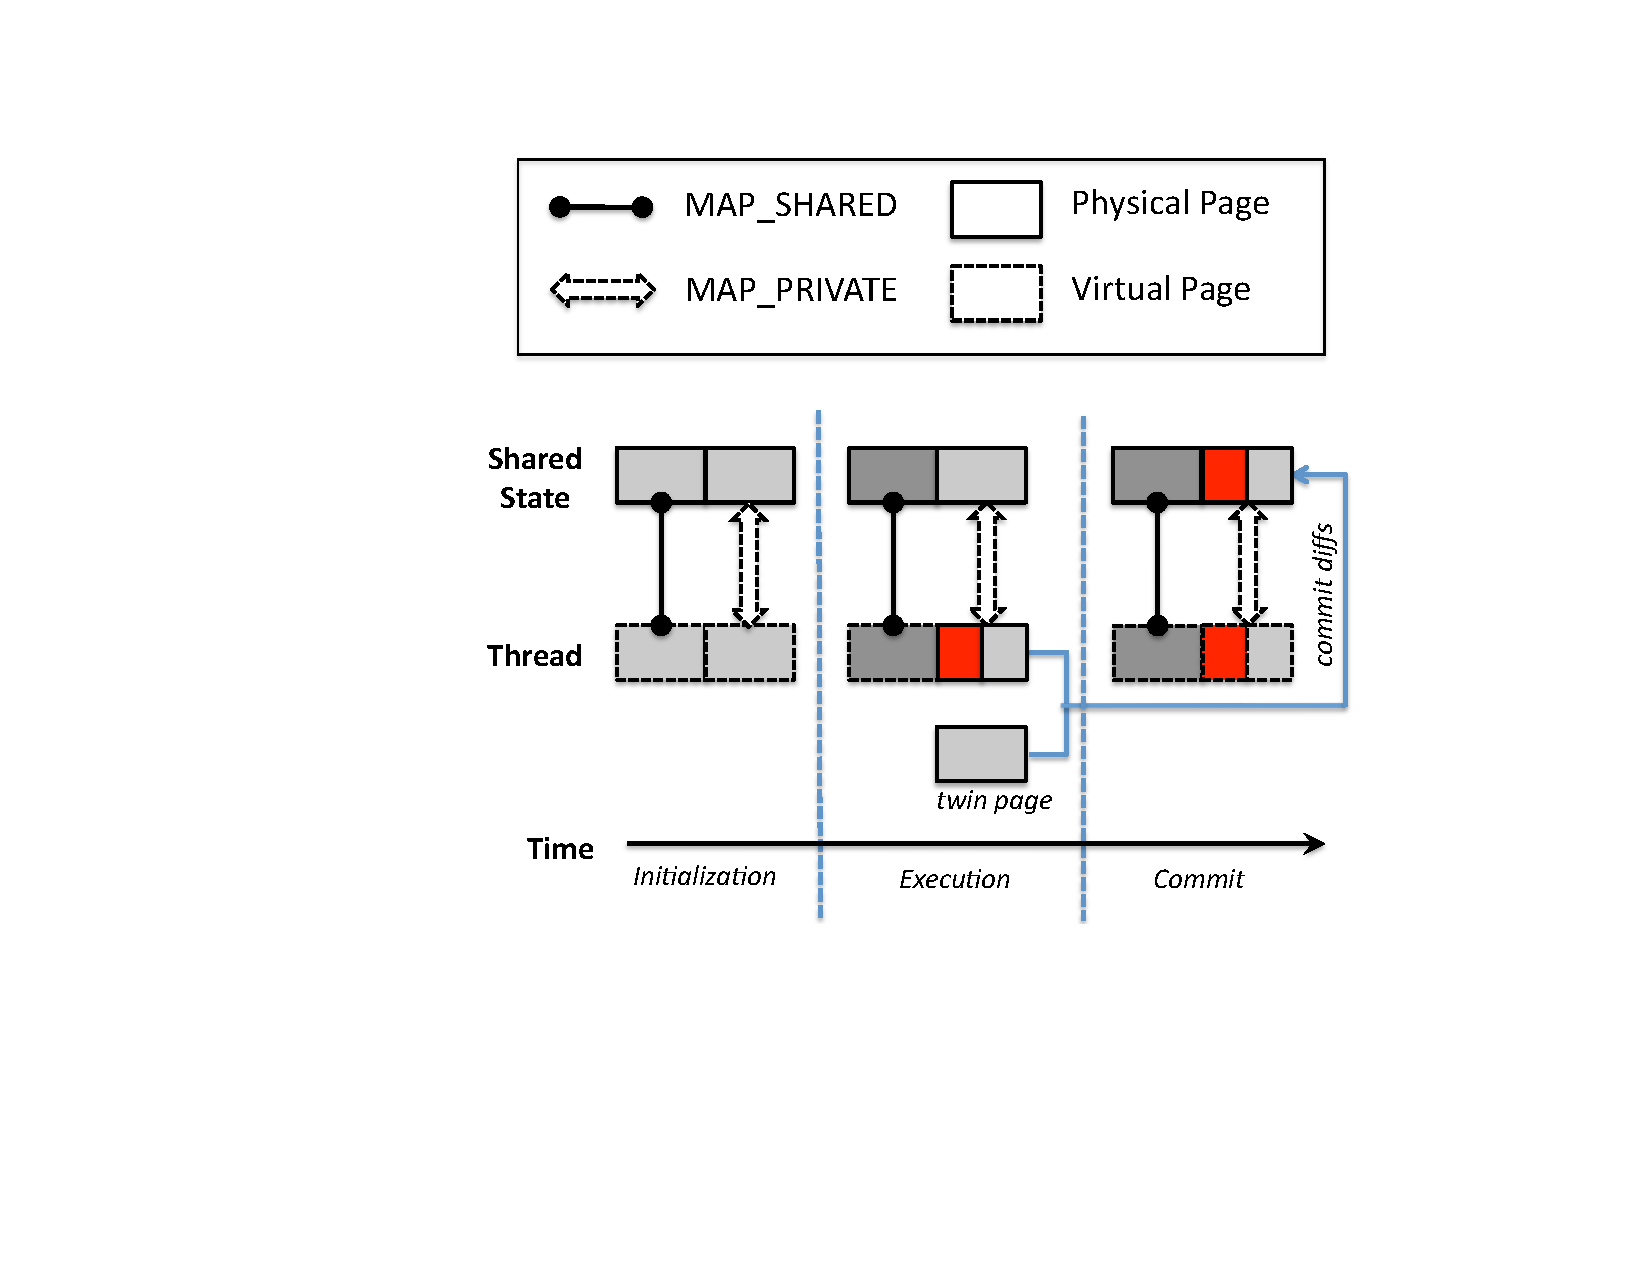
\includegraphics[width=3.5in]{figure/sheriffframework.pdf}
\caption{
\sheriff{} replaces \pthreads{} by simulating threads
with processes. It exposes an API that enables per-thread memory protection and memory isolation on a per-page basis. Each ``thread'' thus either operates directly
on shared memory, or on its own private
copy. For the latter, \sheriff{} commits diffs to shared mappings at synchronization
points (Section~\ref{simulation:syn}).
\label{fig:overview}}
\end{figure}

To create the effect of multi-threaded programs where
different threads share the same address space, \sheriff{} uses
memory mapped files to share the heap and globals across different
processes.  Note that \sheriff{} does not share the stack across
different processes because different threads have their own stacks
and, in general, multithreaded programs do not use the stack for cross-thread
communication.

\sheriff{} creates two different mappings for both the heap and the
globals.  One is a shared mapping, which is used to hold shared state.
The other is a private, copy-on-write (COW) per-process mapping that
each process works on directly.  Private mappings are linked to the
shared mapping through the one memory mapped file. Reads initially go
directly to the shared mapping, but after the first write operation,
both reads and writes are entirely private. \sheriff{}
updates the shared image at synchronization points, as described in
Section~\ref{simulation:thread}.

\sheriff{} uses a fixed-size mapping to hold
globals, which it checks to ensure is large enough to hold all
globals. \sheriff{} also uses a fixed-size mapping to store the heap
(by default, 1GB). Memory allocation requests from user
applications are satisfied from this fixed-size private mapping.

Since different threads allocate memory from this single fixed-size
mapping, the global superheap data structure is shared among different
threads and allocations are protected by one process-based mutex.  In
order to avoid false sharing induced by the memory allocator,
\sheriff{} employs a scalable ``per-thread'' heap organization that is
loosely based on Hoard~\cite{BergerMcKinleyBlumofeWilson:ASPLOS2000}
and built using HeapLayers~\cite{BergerZornMcKinley:2001}.  \sheriff{}
divides the heap into a fixed number of sub-heaps (currently 16).  The
metadata for each sub-heap is also shared by different threads and
protected by a cross-process mutex.  In order to reduce lock
contention, \sheriff{} assigns different sub-heaps to each thread at
creation time. Since each thread's heap allocates from different pages, 
the allocator itself is unlikely to collocate two objects from different 
threads on the same cache line.

Note that tools built with \sheriff{} can specify, on a per-page basis,
whether to use a shared mapping (so that updates are immediately
visible to other ``threads''), or a private mapping (so that updates
are delayed). Both \sheriffdetect{} and \sheriffprotect{} take
advantage of this facility.

\subsection{Shared File Access}
\label{sec:fileshare}

In multithreaded programs, all threads share the same file descriptor table
that tracks the process' open files.  For example, if one thread opens a 
file, the other threads see that the file has been opened.  However, 
multiple processes each have their own resources, including not only 
memory but also file handles, sockets, device handles, and windows.

While \sheriff{} could manage these directly, our current prototype
takes advantage of a feature of Linux that allows selective sharing of
memory and file descriptors. \sheriff{} sets the \texttt{CLONE\_FILES}
flag when creating new processes, resulting in child processes with
different address spaces but the same shared file descriptor table.

\subsection{Synchronization}
\label{simulation:syn}

\sheriff{} supports the full range of POSIX synchronization
operations (mutexes, conditional variables, barriers), as well as all
thread-related calls, including cancellation.

At each synchronization point, \sheriff{} must commit all changes made
by the current thread. The span between
synchronization points thus constitutes a single atomic
transaction. Note that \sheriff{}'s approach differs significantly
from previous transactional memory proposals~\cite{transaction},
including Grace. \sheriff{} is not optimistic, does not replace locks
with speculation (it actually acquires program-level locks), never
needs to roll back (it is always able to commit successfully), and
achieves low overhead for long transactions.

To simulate multithreaded synchronization, \sheriff{}
intercepts all synchronization object initialization function calls,
allocates new synchronization objects in a mapping shared
by all processes, and initializes them to be accessible by different
processes.

\sheriff{} wraps
all synchronization operations, including mutexes, condition
variables, and barriers in a similar fashion. For example, a call to
\texttt{pthread\_mutex\_lock} first ends the current transaction, 
then calls the corresponding \pthreads{} library function but on a
cross-process mutex. \sheriff{} then starts a new transaction after the
lock is acquired, which ends with the next synchronization operation.

Thread-related calls are implemented in terms of their process
counterparts. For example, \texttt{pthread\_join} ends the current
transaction and calls \texttt{waitpid} to wait for the appropriate
process to complete.


\subsection{Updating Shared Memory}

\label{sec:updatingsharedmemory}

At each synchronization point, \sheriff{} updates the shared
globals and heap with any updates that thread made.  To accomplish
this \sheriff{} uses \emph{twinning} and \emph{diffing}, mechanisms
first introduced in distributed shared memory systems to reduce
communication overhead~\cite{dsm:munin,dsm:treadmarks}.

% CC: Removed this, since diffs are always used to identify modifications
% \sheriffdetect{} uses diffs to identify modifications.

Figure~\ref{fig:overview} presents an overview of both mechanisms at
work. All private pages are
initially write-protected. Before any page is modified, \sheriff{}
copies its contents to a ``twin page'' and then unprotects the
page. At a synchronization point, \sheriff{} compares each twin page
to the modified page (byte by byte) to compute diffs.

\subsection{Example Execution}
\label{simulation:thread}

This section walks through an example of \sheriff{}'s execution from the start of a program to its termination.

% Figure~\ref{fig:overview} presents an overview of \sheriff{}'s execution.

\paragraph{Initialization: } Before the program begins, \sheriff{}
establishes the shared and local mappings for the heap and globals,
and initiates the first transaction.

\paragraph{Transaction Begin:}
At the beginning of every transaction, \sheriff{} write-protects any shared
pages so that later writes to these pages can be caught by
handling \texttt{SEGV} protection faults.  In later transactions,
\sheriff{} only write-protects pages dirtied in the last
transaction, since the others remain write-protected.

\paragraph{Execution: } While performing reads, \sheriff{} runs at
the same speed as a conventional multithreaded
program. However, the first write to a protected page triggers a page
fault that \sheriff{} handles.

\sheriff{} records the page holding the faulted address and then unprotects
this page so that future accesses run at
full speed.  Each page thus incurs at most one page fault per transaction.
Although protection faults and signals are expensive, these costs are
amortized over the entire transaction.

However, before servicing the fault, \sheriff{} must first obtain an
exact copy of this page (its twin). \sheriff{} accomplishes this by
forcing a copy-on-write operation on this page by writing to the start
of this page with contents from the same address (i.e., it
reads and writes the same value).

This step is essential to ensure that the twin is identical to the
original, unmodified page. After the signal handler, the OS's
copy-on-write mechanism creates a new, private page.

\paragraph{Transaction End: } At the end of each atomically-executed
region---at thread exit and before synchronization
points---\sheriff{} commits changes from
private pages to the shared space and reclaims memory holding old
private pages and twin pages.

\sheriff{} commits only the differences between the twin and the
modified pages. Once it has written these diffs, \sheriff{} issues an
\texttt{madvise} call with the \texttt{MADV\_DONTNEED} flag that
discards the physical pages backing both the private mapping and the
twin pages. This action allows the OS to reclaim this memory, helping
to ensure that \sheriff{}'s memory overhead remains close to that of
the original program.

\subsection{Discussion}

As Section~\ref{simulation:sharememory} notes, \sheriff{} does not
share the stack between different threads. When using \pthreads{},
threads are allowed to share stack variables with their parent.
As long as threads do not modify these variables,
\sheriff{} operates correctly. However, \sheriff{} does not preserve
\pthreads{} semantics for applications whose threads
\emph{modify} stack variables from their parent thread that their
parent then reads. Fortunately, passing stack variables to a thread
for modification is generally frowned upon, making it a rare coding
practice.

\sheriff{} cannot currently intercept atomic operations
written in assembly, so programs that implement their own
\emph{ad hoc} synchronization operations are not guaranteed to work
correctly (Xiong et al.\ have shown that 22--67\% of the uses of
\emph{ad hoc} synchronization they examined led to bugs or severe
performance issues~\cite{ad-hoc-considered-harmful}). We expect this
limitation to be less of a problem in the future because the
forthcoming C++0x standard exposes atomic operations in a standard
library, making it possible for \sheriff{} to intercept them.


\chapter{\dthreads{}:Efficient Deterministic Multithreading}
% How to implement the deterministic threads.
\Dthreads{} is built on \Sheriff{} framework to support deterministic executions of
multithreaded programs:  a program with the same input always has the same execution and 
the same output.
\Dthreads{} is also a drop-in replacement of the \pthreads{} library:
users don't need to change their programs, 
to recompile their programs, nor to change the underlying operating
systems. \dthreads{} automatically provides the determinism for programs if they are linked to 
\dthreads{} library directly or using LD\_PRELOAD mechanism.

To support the deterministic running of a program, 
\Dthreads{} breaks the whole execution into intermittent parallel phases and serial phases 
(see Figure~\ref{fig:dthreadsphases}) based on explicit synchronization calls of a program: 
program sections without synchronizations are running in parallel 
phases and others are running in serial phases.
Synchronizations are those ways to communicate across different threads, 
including thread creation and exit; mutex lock and unlock; conditional variable wait
and signal; posix sigwait and signal; and barrier wait. 

In parallel phases, thread executions are running in the isolation mode, which is discussed 
in detail in Section~\ref{sec:dthreadsisolation}.
In serial phases, updates from different threads are exposed to other threads 
in a deterministic order and deterministic synchronizations are performed, which are 
discussed in Sections~\ref{sec:dthreadsdeterm}. 

\begin{figure}[b]
{\centering 
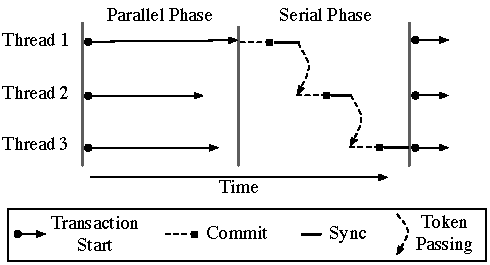
\includegraphics{fig/phase-diagram} 
\caption{Overview of \dthreads{} phases
\label{fig:dthreadsphases}}
}
\end{figure}

\section{Isolated Memory Accesses}
\label{sec:dthreadsisolation}

\Sheriff{} framework provides a ``per-thread-isolation'' mechanism, isolating the executions
of different threads relying on different address spaces of processes.
\dthreads{} utilizes this isolation mechanism to localize different threads' modifications in
parallel phases: 
updates of each thread can not be seen by other threads and a thread can only observe those 
changes made by itself in the program order. 
Inside a parallel phase, the execution is not intervened by those executions from other threads 
so it is guaranteed to be deterministic. 

\section{Deterministic Memory Updates and Synchronizations}
%In the serial phases, updates from different threads are exposed in a deterministic order and deterministic synchronizations are performaned. We discussed these mechanisms in Sections~
\label{sec:dthreadsdeterm}
Since multithreaded programs often use shared memory to communicate, 
\dthreads{} must expose one thread's modifications 
to other threads at synchronization points deteriminically in order to ensure 
the deterministic execution.
%, these updates must be applied at deterministic times, and in a deterministic order.
%\dthreads{} exposed those modifications to the shared mapping in sequence 
%at synchronization points.
 
However, those local modificatons can not be exposed immediately when a thread reaches a 
synchronization point: committing local updates to the shared mapping should not
change the views of memory state for other threads. 
In order to guarantee the determinism, \dthreads{} introduces an internal fence: 
a thread only commits its local modifications after all other threads reach 
the same internal fence. 
This fence is similar to the barrier mechanism of \pthreads{}.  
We re-implemented this since
\pthreads{} barrier can not support the change of waiters number dynamically.

In order to avoid races in commit procedures, those commits must be performed in a 
deterministic order: 
\dthreads{} invents a global token to pass across differnt threads in a round-robin way  
and a thread can only commit its local modifications when holding the token.

The order to pass token is set to the order of threads creation initially but can be changed 
in some cases: 
when a thread is waiting on conditional variables, this thread will be taken out of the list 
of token passing; it will be put to the list again when waken up from conditional wait. 
Also, synchronizations are performed by utilizing this global token too: a thread can perform 
synchronizations when it holds the token. 

It is possible to encounter the deadlock problem when a thread holding multiple locks 
performs locks one by one using this global token. 
\dthreads{} treats multiple locks as a single lock: the token is passed to next thread when all locks
are released. 

\section{Conclusion}

Comparing to previous deterministic multithreading, 
\Dthreads{} provides a stable deterministic multithreading even in
the faces of data races: executions of a program always behave the same, even with different inputs or 
on different hardware, as long as the synchronization order is staying the same. \Dthreads{} 
dramatically improves the performance of the state-of-the-art (CoreDet~\cite{coredet}) by
3.4$\times$ without resorting to any hardware change.
In this work, \dthreads{} novelly implements a deterministic memory allocator, which can
guarantee the determinsim even for programs with memory errors, such as buffer overflows.  

However, \dthreads{} suffers from the same shortcoming as that of \sheriff{}: those programs
with ad hoc synchronization may not work properly since \dthreads{} does not commit 
those modifications of ad hoc synchronization, which needed by synchronization, 
without explicit instrumention and annotation.
\dthreads{} can also suffer the load imbalance problem of explicit synchronization 
points of programs, 
which can still guarantee the determinism but may compromise the performance.
%\coreDet{}:. 

% Why it is performing well.
% Deterministic memory allocation. 
% What is the shortcoming: can't work for the ad-hoc synchronization. The performance may encounter the 
% load-balance problem. 


\chapter{Proposed Work: Locate Memory Errors Efficiently and Precisely}
% Experience from Grace, which are utilizing the rollback mechanism to avoid 
% memory conflict.
% During the development of \sheriff{}, we actually find out some race problems of program in
% the commit phase. 
% Now we are trying to bind all those together: utilize the rollback and watch point to find out
% memory errors.
% The idea is actually the same: only check memory errors in some points, intead of every access,
% we can actually improve the performance of memory debugging system. 
We propose \stopgap{} system to locate the memory errors of 
multithreaded programs precisely and efficiently, such as write-write races and buffer overflows. 

\section{Detection of Write-Write Races}

% How to find out the write-write race conditions
Since \Sheriff{} can determine actual 
modifications of different threads by combining
``per-thread-isolation'', ``per-thread-protection'' and ``twinning-and-diffing'' mechanism
altogether, \stopgap{} leverages this framework to detect write-write races.
 
The basic idea of \stopgap{} to find out the write-write races is as follows: 
whenever a thread finds those modifications before actual commits, 
it snoops the shared mapping to check whether the shared mapping has a different value 
with that of the twin page.
%If the shared mapping has a different value with that of the twin
%page, other threads must change this word simultaneously with current thread. 

Ideally, accessing a shared variable must be protected by a mutual exclusion lock, 
so two threads can not enter into the same critical section simultaneously.
It is impossible for a correctly synchronized program that two threads modify 
the same word simultaneouly.  
If a word is changed by multiple threads simultaneously, it can only be caused by a race.
Because \stopgap{} preserves the same synchronization semantics of multithreaded programs, 
two threads modifying the same word simultaneously must be caused by a write-write race.
Because of that, \stopgap{}  never reports false 
positives: those write-write races are actually races. 

Since \stopgap{} only checks memory accesses and commits per-thread's modifications 
at synchronization 
boundaries and system calls, it is expected to greately amortize the overhead 
through a long period of time. 
%and to avoid the skews of executions by the logging mechanism:
Different with traditional approaches, there is no need to record every memory access and its 
corresponding timing information, which can also reduce the space overhead of detection tools. 

%\textbf{AAAA}
% Why \stopgap{} can find more races?
In the meanwhile, \stopgap{} possibly detects more races since all updates in the 
in the same epoch can be found out by examining the difference between the shared 
mapping and the twin page.
We do not need to detect a race when two accesses actually violate the happens-before 
relationship any more.

However, simply knowing a race is not helpful for users to fix this problem. 
In order to precisely locate the problem, \stopgap{} is planning to combine the program
re-execution and watch point mechanism to find out the origins of the problem.
The basic mechanism is showed in Figure~\ref{fig:stopgapoverview}: 
\stopgap{} first snapshots the program before its running; then the program can run at 
full speed until the end of a program, at system calls or at synchronization boundaries;
\stopgap{} only check memory accesses accumulatively at the end of a program, at system calls and 
synchronization boundaries,  so \stopgap{} amortizes
the snapshot and checking overhead over a long execution.
\stopgap{} only pays the overhead to re-execute a program when a program has some memory errors. 
In order to capture context of problematic memory accesses precisely and efficiently,
\stopgap{} installs the hardware watchpoint on those problematic addresses(~\ref{sec:watchpoint})
before a program with memory errors is re-executed(~\ref{sec:re-execute}).
%\stopgap{} re-executes a program deterministically by
%utilizing the snapshot of a program in the beginning and rolls back
%the program to a stored state.

\begin{figure}[!t]
{\centering
\includegraphics[width=5.4in]{fig/stopgapoverview2}
\caption{Overview of \stopgap{}
\label{fig:stopgapoverview}}
}
\end{figure}

% What is the rollback mechanism
\subsection{Re-execution of A Program}
\label{sec:re-execute}
\stopgap{} targets to locate those overflows precisely using the re-execution,
thus it is important for \stopgap{} to repeat the initial execution:
those overflows and races happening in the initial execution should happen exactly the same in
the re-execution phase, on the same addresses and with the same behavior.
In order to achieve this target, 
we are planning to utilize the \dthreads{} framework for determinism support.  

% What is the watch point mechanism
\subsection{Watch Point Mechanism}
\label{sec:watchpoint}

Watch point mechanism is using hardware debug registers to watch the memory accesses on
some specific addresses. Some previous works have used this mechanism 
for their specific targets \cite{fastboundschecking}. 
Debug register hardware is universally supported by most if not all existing CPUs, such as
X86 and X86-64 architecture, PowerPC, MIPS, ARM, etc. 
Generally, this watch point technique can support the memory watching efficiently: whenever
a memory access matches one of those debugging address, the user can be notified by an exception.
% What is the basic idea of \stopgap{}.

\section{Buffer Overflow}
Those existing mechanisms to find out buffer overflow problems either can not pinpoint the origins of
problems precisely or their performance overhead is too high to be deployed. 
Those traditional approaches pinpointting the origins of problems should 
check every memory access in order to capture those accesses beyond the scope of 
current memory block. 
If a buffer overflow is found, the program will be stopped immediately 
so that user can find out where the problem occurs.
Thus, this kind of approach is also called as ``stop-and-report'' approach here. 

However, ``stop-and-report'' approach introduces significant performance overhead by 
checking every memory access,  
preventing their usage in actual deployed environment. 
We propose to utilize the \stopgap{} mechanism (described in the above section) 
to detect buffer overflows and underflows efficiently. 

In order to detect those overflows, \stopgap{} puts one guard zone before and 
one after each heap object. \stopgap{} initializes all guard zones to a pre-known special 
value when a heap object is allocated.
When buffer overflow occurs, values of guard zones must be changed to a different value.
By detecting the changes of guard zones, \stopgap{} can detect the buffer overflows. 
%Since \stopgap{} greately reduces the number of checkings, the overhead
%is expected to be largely amortized over a long execution time.
%\stopgap{} can report more information than the traditional stop-and-report approach:
%\stopgap{} can provide the whole access sequence
%on some specific addresses, which can help to identify the actual
%problems in the complex systems.
Same as the mechanisms to locate the write-write races, \stopgap{} only checks overflows 
in the end of a program or at synchronization boundries, hoping to greately reduce
the overhead.  
\stopgap{} also utilizes the rollback mechnism and watch point mechanism to find
the origins of overflows precisely.

\subsection{Preliminary Results}
We have finished a practical buffer overflow detection tool for single-threaded program, which only
introduces minor performance overhead (about 5\%), much lower than the state-of-the-art technique.
The state-of-the-art tool to detect the buffer overflow problem,
AddressSanitizer from \texttt{Google}, introduces about 26\% performance overhead.

% What is the challenge here?
\section{Schedule and Delieverables}

The proposed timeline for this thesis is as follows:

\begin{table}[ht]
\centering
\begin{tabular}{ l r}
Implementing the basic machanism of \stopgap{} & March 2013 \\ 
Evaluating the performance and effectiveness & May 2013 \\
Improving the performance and effectiveness & June 2013 \\
Thesis chapter drafts & May 2013 \\ 
Paper submitted to ASPLOS & July 2013 \\
Thesis defense  & Summer 2013\\
Graduate & Summer 2013 \\
\end{tabular}
{\label{table:timeline}}
\end{table}

For this thesis work, ideally, a paper would be submitted to ASPLOS conference in July 2013. 
Corresponding code will be publicize on GitHub, so that people can utilize the software
derived from this thesis work
to detect the race conditions and buffer overflows in multithreaded programs.


%%
%% Beginning of back matter
\backmatter  %% <--- mandatory

%%
%% We don't support endnotes

%%
%% A bibliography is required.
\bibliographystyle{umthesis}
\bibliography{refs}
\end{document}

%%% Local Variables: 
%%% mode: latex
%%% TeX-master: t
%%% End: 
